% Options for packages loaded elsewhere
\PassOptionsToPackage{unicode}{hyperref}
\PassOptionsToPackage{hyphens}{url}
\documentclass[
]{book}
\usepackage{xcolor}
\usepackage{amsmath,amssymb}
\setcounter{secnumdepth}{5}
\usepackage{iftex}
\ifPDFTeX
  \usepackage[T1]{fontenc}
  \usepackage[utf8]{inputenc}
  \usepackage{textcomp} % provide euro and other symbols
\else % if luatex or xetex
  \usepackage{unicode-math} % this also loads fontspec
  \defaultfontfeatures{Scale=MatchLowercase}
  \defaultfontfeatures[\rmfamily]{Ligatures=TeX,Scale=1}
\fi
\usepackage{lmodern}
\ifPDFTeX\else
  % xetex/luatex font selection
\fi
% Use upquote if available, for straight quotes in verbatim environments
\IfFileExists{upquote.sty}{\usepackage{upquote}}{}
\IfFileExists{microtype.sty}{% use microtype if available
  \usepackage[]{microtype}
  \UseMicrotypeSet[protrusion]{basicmath} % disable protrusion for tt fonts
}{}
\makeatletter
\@ifundefined{KOMAClassName}{% if non-KOMA class
  \IfFileExists{parskip.sty}{%
    \usepackage{parskip}
  }{% else
    \setlength{\parindent}{0pt}
    \setlength{\parskip}{6pt plus 2pt minus 1pt}}
}{% if KOMA class
  \KOMAoptions{parskip=half}}
\makeatother
\usepackage{longtable,booktabs,array}
\usepackage{calc} % for calculating minipage widths
% Correct order of tables after \paragraph or \subparagraph
\usepackage{etoolbox}
\makeatletter
\patchcmd\longtable{\par}{\if@noskipsec\mbox{}\fi\par}{}{}
\makeatother
% Allow footnotes in longtable head/foot
\IfFileExists{footnotehyper.sty}{\usepackage{footnotehyper}}{\usepackage{footnote}}
\makesavenoteenv{longtable}
\usepackage{graphicx}
\makeatletter
\newsavebox\pandoc@box
\newcommand*\pandocbounded[1]{% scales image to fit in text height/width
  \sbox\pandoc@box{#1}%
  \Gscale@div\@tempa{\textheight}{\dimexpr\ht\pandoc@box+\dp\pandoc@box\relax}%
  \Gscale@div\@tempb{\linewidth}{\wd\pandoc@box}%
  \ifdim\@tempb\p@<\@tempa\p@\let\@tempa\@tempb\fi% select the smaller of both
  \ifdim\@tempa\p@<\p@\scalebox{\@tempa}{\usebox\pandoc@box}%
  \else\usebox{\pandoc@box}%
  \fi%
}
% Set default figure placement to htbp
\def\fps@figure{htbp}
\makeatother
\setlength{\emergencystretch}{3em} % prevent overfull lines
\providecommand{\tightlist}{%
  \setlength{\itemsep}{0pt}\setlength{\parskip}{0pt}}
\usepackage[]{natbib}
\bibliographystyle{apalike}
\usepackage{booktabs}
\usepackage{amsthm}
\makeatletter
\def\thm@space@setup{%
  \thm@preskip=8pt plus 2pt minus 4pt
  \thm@postskip=\thm@preskip
}
\makeatother
\usepackage{bookmark}
\IfFileExists{xurl.sty}{\usepackage{xurl}}{} % add URL line breaks if available
\urlstyle{same}
\hypersetup{
  pdftitle={Manual de usuario de MonitorEO-OBSNEV},
  pdfauthor={Observatorio de Cambio Global de Sierra Nevada (Universidad de Granada)},
  hidelinks,
  pdfcreator={LaTeX via pandoc}}

\title{Manual de usuario de MonitorEO-OBSNEV}
\author{Observatorio de Cambio Global de Sierra Nevada (Universidad de Granada)}
\date{2025-02-27}

\begin{document}
\maketitle

{
\setcounter{tocdepth}{1}
\tableofcontents
}
\chapter{Introducción}\label{intro}

MonitorEO-OBSNEV es una herramienta de análisis de variables derivadas de teledetección satelital basada en Google Earth Engine desarrollada por el Observatorio de Cambio Global de Sierra Nevada (Universidad de Granada).

\chapter{Interfaz gráfica}\label{interfaz}

Estás dentro del \textbf{Laboratorio de Investigación Virtual MonitorEO-OBSNEV} (Monitoring with Earth Observations del OBServatorio de Cambio Global de Sierra NEVada), un \textbf{sistema de seguimiento y alerta basado en teledetección,} diseñado para monitorizar cambios en \textbf{variables esenciales de la biodiversidad} relacionadas con el funcionamiento y la estructura de los ecosistemas en cualquier parte del mundo.

\pandocbounded{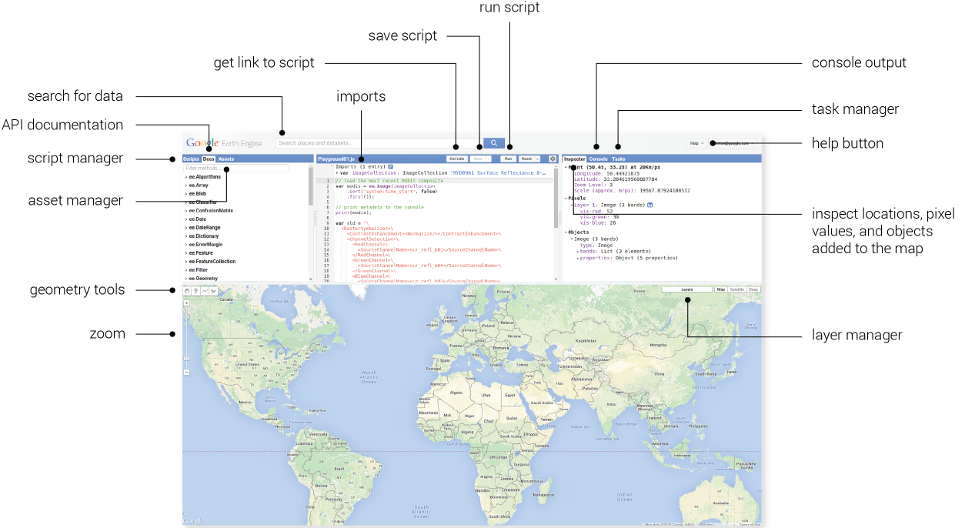
\includegraphics[keepaspectratio]{assets/annotated_playground.png}}

\chapter{Idiomas}\label{idiomas}

\textbf{Selecciona el idioma} de la interfaz: encontrarás disponibles es-español, en-english y ds-alemán.

\chapter{Área de estudio}\label{area-estudio}

\textbf{Selecciona ROI:} Elige tu área de estudio. Dentro de esta sección podrás:

\begin{itemize}
\tightlist
\item
  \textbf{Dibujar tu región de interés (ROI - Region of Interest).} Puedes dibujar regiones manualmente usando esta opción. Cuando dibujas una región (punto, línea o polígono), esta se almacena como un objeto Geometry que aparecerá como capa en la parte superior izquierda del mapa.\\
\item
  \textbf{Punto específico y radio.} Puedes introducir las coordenadas de latitud y longitud de una ubicación específica en la superficie terrestre. El radio se usa comúnmente en buffers, que son áreas circulares alrededor de un punto. MonitorEO-OBSNEV permite crear un buffer alrededor de un punto con un radio específico en kilómetros.\\
\item
  \textbf{Elige un proyecto.} Puedes utilizar el área de estudio de los distintos proyectos de OBSNEV.

  \begin{itemize}
  \tightlist
  \item
    \textbf{EarthCul:} Área de influencia socioeconómica de Parques Nacionales de Montaña de España y Portugal.\\
  \item
    \textbf{EVEREST}: Parques Nacionales de Montaña de España y Portugal.\\
  \item
    \textbf{PRESINMED}:\\
  \item
    \textbf{BioRefuges}
  \end{itemize}
\end{itemize}

Hay que añadir las áreas de estudio PRESINMED y BioRefuges

\chapter{Fechas de inicio y fin}\label{fechas}

Elige el rango de fechas para realizar tus cálculos. Primero, establece el \textbf{año de inicio} y el \textbf{año de fin}. Luego, selecciona el \textbf{mes y día de inicio}, así como el \textbf{mes y día de finalización} para definir el período de análisis.

\chapter{Selección de un intervalo de meses específico}\label{periodo}

Al activar la casilla \textbf{``Solo intervalo MM/DD a lo largo de los años''} se realiza un \textbf{cómputo estacional}, es decir, se establece un rango temporal específico dentro del periodo de años seleccionado previamente. P.ej. todas las primaveras de 2001 a 2020 (Año inicio 2001 - Año fin 2020, Desde 21/03 - Hasta 21-09).

\chapter{Tipo de variable de interés}\label{tipo-variable}

Selecciona la variable de estudio. Las variables se clasifican en grandes categorías de \href{https://geobon.org/ebvs/what-are-ebvs/}{EBVs} \textbf{(Variables Esenciales de Biodiversidad)}, relacionadas con el funcionamiento y estructura de los ecosistemas. \textbf{MonitorEO-OBSNEV} incluye:

\begin{itemize}
\tightlist
\item
  \textbf{Carbono Orgánico (Producción Primaria):}

  \begin{itemize}
  \tightlist
  \item
    \textbf{NDVI} - Normalized Difference Vegetation Index.\\
  \item
    \textbf{EVI} - Índice de Vegetación Mejorado.\\
  \item
    \textbf{Chl-a} - Concentración de clorofila.\\
  \end{itemize}
\item
  \textbf{Balance de Radiación:}

  \begin{itemize}
  \tightlist
  \item
    \textbf{ALB} - Albedo.\\
  \end{itemize}
\item
  \textbf{Balance de Agua:}

  \begin{itemize}
  \tightlist
  \item
    \textbf{ET} - Evapotranspiración\\
  \item
    \textbf{LE} - Calor Latente\\
  \item
    \textbf{LSWI} - Índice de Agua Superficial Terrestre\\
  \item
    \textbf{NDWI} - Índice de Agua de Diferencia Normalizada\\
  \item
    \textbf{NDSI} - Índice de Nieve de Diferencia Normalizada\\
  \end{itemize}
\item
  \textbf{Calor Sensible:}

  \begin{itemize}
  \tightlist
  \item
    \textbf{LST} -Temperatura Superficial.\\
  \end{itemize}
\item
  \textbf{Nutrientes / Aerosoles:}

  \begin{itemize}
  \tightlist
  \item
    \textbf{ARSL} - Profundidad óptica atmosférica de aerosoles.
  \end{itemize}
\end{itemize}

Añadimos la descripción detallada de cada índice? la tengo \href{https://docs.google.com/document/d/1iYMDXfh4uQ9vuNyansFqoBuk0M9Hi5Vo_4U-cOyEGcY/edit?tab=t.0}{\textbf{aquí}}

\chapter{Variable específica}\label{variable-especifica}

xxx

\chapter{Sensor satelital}\label{sensor}

Selecciona con qué sensor quieres trabajar. Los sensores disponibles poseen distinta resolución temporal y espacial. Dependiendo de la variable elegida, obtendrás disponibilidad de datos para unos u otros sensores. Todos sensores disponibles son:

\begin{itemize}
\tightlist
\item
  \textbf{MODIS 250 m, 16 días.} MODIS (\emph{Moderate Resolution Imaging Spectroradiometer}) es un sensor a bordo de los satélites Terra y Aqua de la NASA. \textbf{Resolución espacial:} 250 metros (m). \textbf{Resolución temporal:} 16 días (se compilan imágenes cada 16 días en productos de composición).\\
\item
  \textbf{Landsat 30 m, \textgreater{} 8 días.} La serie \textbf{Landsat} es operada por la NASA y el USGS. Estos datos incluyen Landsat 5, 6, 8 y 9. \textbf{Resolución espacial:} 30 metros. \textbf{Resolución temporal:} Mayor a 8 días, ya que dependiendo del satélite tienen un período de revisita de 8 o 16 días cada uno.\\
\item
  \textbf{Sentinel-2 10m, 5 días}. El programa \textbf{Sentinel-2} es operado por la Agencia Espacial Europea (ESA) y forma parte del programa Copernicus. \textbf{Resolución espacial:} 10 metros. \textbf{Resolución temporal:} 5 días.
\end{itemize}

\chapter{Unidad temporal de agregación}\label{agregacion-temporal}

Elige la resolución temporal para tus cálculos: puedes mantener la resolución original del sensor, cada 16 días, agrupar los datos por mes o por año.

\chapter{Métrica de agregación espacial}\label{agregacion-espacial}

Selecciona el método de agregación espacial para ejecutar tu análisis. Los métodos de \textbf{agregación espacial} permiten \textbf{resumir datos} en áreas utilizando diferentes técnicas estadísticas llamadas \textbf{reductores}.

\begin{itemize}
\tightlist
\item
  \textbf{Media:} Calcula el \textbf{promedio} de los valores dentro del período de tiempo seleccionado.\\
\item
  \textbf{Mediana}: Calcula el \textbf{valor central} en un conjunto de datos ordenados. Es más resistente a valores extremos que la media.\\
\item
  \textbf{Moda:} Calcula el \textbf{valor más frecuente} en un conjunto de datos.\\
\item
  \textbf{Mínimo:} Calcula el \textbf{valor más bajo} en un período de tiempo.\\
\item
  \textbf{Máximo:} Calcula el \textbf{valor más alto} en un período de tiempo.\\
\item
  \textbf{Percentil 10:} Encuentra el valor por debajo del cual está el \textbf{10\% de los datos}. Se usa para medir \textbf{valores bajos} o eventos extremos.\\
\item
  \textbf{Percentil 90:} Encuentra el valor por debajo del cual está el \textbf{90\% de los datos}. Se usa para medir \textbf{valores altos} o eventos extremos.
\end{itemize}

\chapter{Filtrado de nubes}\label{filtrado-nubes}

Al activar esta casilla, se aplicará un \textbf{filtrado de nubes por escena}. El filtrado de nubes por escena es un proceso utilizado en el análisis de imágenes satelitales para eliminar o reducir la interferencia causada por la presencia de nubes en cada imagen, mejorando la calidad de los datos. Como resultado, los análisis reflejarán con mayor precisión las características reales de la superficie terrestre.

\chapter{Generar mapas y gráficos de resultados}\label{mapas-graficos}

Al hacer clic en el botón \textbf{``Calcular''}, se generará el resultado según tu selección previa.

En la sección \textbf{``Set.Layer''}, aparecerán todas las capas o mapas generados durante el cálculo. Para visualizar una capa específica, selecciónala en \textbf{``Set.Layer''} y haz clic en \textbf{``Añadir''}.

Para ver los gráficos asociados a los resultados, selecciona la opción \textbf{``Chart''}.

Por completar, aclarar con Pablo cómo se le daba para mostrar cada tipo de gráfico

\bibliography{book.bib,packages.bib}

\end{document}
